\documentclass[11pt,letterpaper,headsepline,pagesize,letterpaper,DIV12,liststotoc]{scrartcl}
\usepackage[T1]{fontenc}
\usepackage{graphicx,verbatim,rotate,times,subfigure}
\usepackage{longtable}
\usepackage[latin1]{inputenc}
% paragraph setup
\setlength{\parindent}{0pt}
\setlength{\parskip}{0.4\baselineskip plus1pt minus1pt}
% not in this country: \frenchspacing
%
% page setup
%
\usepackage[automark]{scrpage2}
\pagestyle{scrheadings}
\renewcommand{\headfont}{\normalfont\sffamily}
\renewcommand{\pnumfont}{\normalfont\sffamily}
\clearscrheadfoot
\ohead{\pagemark}\chead{}\ihead{\headmark}
\ofoot{}\cfoot{}\ifoot{}
\pagestyle{scrheadings}
\thispagestyle{empty}
%\ohead{\pagemark}\chead{}\ihead{\headmark}\cfoot{}
%
% I hate koma's page layout, so I fix it my way
%
%\setlength{\topmargin}{0pt} % headexclude document style is broken
\setlength{\textheight}{1.08\textheight} % add n% more length
\setlength{\textwidth}{1.05\textwidth} % add n% more width
%
% my verbatim stuff
%
\makeatletter
\newlength{\myverbatimindent}
\setlength{\myverbatimindent}{10mm}
\renewcommand{\verbatim@processline}{%
  \leavevmode\hspace*{\myverbatimindent}\the\verbatim@line\par}
\renewcommand{\verbatim@font}{\bf\ttfamily\small\baselineskip10pt}
\makeatother
%
% personal shortcuts
%
\font\manual =manfnt scaled \magstep0
\def\dbend{{\manual\symbol{127}}}
%
\newenvironment{difficult}%
  {{\makebox[-50pt][r]{\raisebox{8pt}{\dbend}}\makebox[50pt][l]{}}%
   \small\leftskip5mm}%
  {\par\normalsize\leftskip0pt}
%
\def\bs{$\mathbf{\backslash}$}
\def\dd{\\\hline}
\def\at{\symbol{64}}
\def\ul#1{\underline{#1}}
\def\rref#1{\ref{#1} (page~\pageref{#1})}
%
% should be last
%
\usepackage{hyperref}
%
%
\title{Kickstart V2}
\date{06/06/2004}
\author{Jens-S. V�ckler}
%
\usepackage{hyperref}
%
\begin{document}
\thispagestyle{empty}
\maketitle
\begin{center}
  \begin{tabular}{|l|l|p{80mm}|}\hline
    \textbf{Author} & \textbf{Date} & \textbf{Modification}\dd\hline
    Jens V�ckler & 20040204 & initial document\dd
    Jens V�ckler & 20040211 & extensions\dd
    Jens V�ckler & 20040607 & added \texttt{here} to stdin, and setup
    jobs\dd 
  \end{tabular}
\end{center}
\setlongtables
\pagebreak
\tableofcontents
\vfill
\begin{difficult}
Difficult sections which are not important for the casual users are
expressed with a dangerous bend sign in the margin.  
\end{difficult}
\pagebreak

\section{Overview}
\label{sec:overview}

Kickstart is a grid shell. A grid shell is run at the remote execution
host, and like a shell, starts and watches over an application.
Figures~\ref{fig:without} and~\ref{fig:with} compare the absence and
presence of a grid shell in the remote job execution chain.

\begin{figure}[htbp]
  \centering
  \includegraphics{without}
  \caption{Without the presence of a grid shell.}
  \label{fig:without}
\end{figure}

\begin{figure}[htbp]
  \centering
  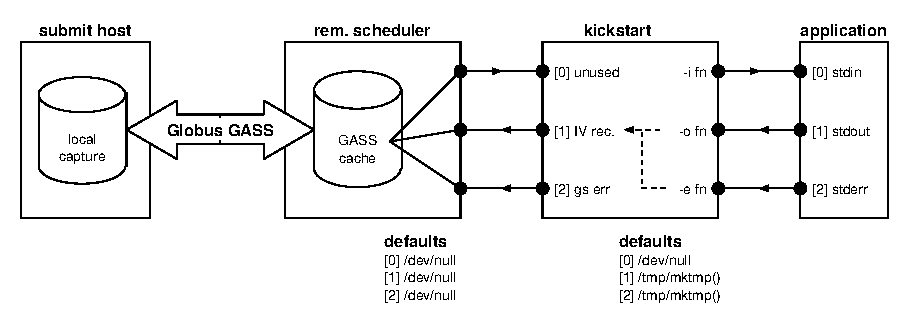
\includegraphics{with}
  \caption{With the presence of kickstart.}
  \label{fig:with}
\end{figure}

In the absence of a grid shell, figure~\ref{fig:without}, the remote
scheduler starts the application on any worker. The stdio streams of the
application usually default to either \verb|/dev/null| or some other
scheduler-specific file. Through the presence of Globus, stdio can be
both, streamed or staged, via GASS. Furthermore, the application itself,
if independently bundled (i.e. statically linked), and appropriate for
the architecture, can be staged using GASS from the submit site.

In the presence of a grid shell, figure~\ref{fig:with}, specifically
kickstart, the GASS-handled stdio streams are used for kickstart's own
purposes. Since kickstart is used in conjunction with the GriPhyN
Virtual Data System (GVDS), any application stdio streams are known and
registered with the GVDS. If a stream is important to an application,
e.g. the application produces results on \emph{stdout}, the stream can
be connected to a file on the remote system. The GVDS will generate the
right configuration to have a grid shell locally connect the stream to a
file on the remote machine.

Although kickstart provides the capture of stdio of remote application,
the GVDS-tracked stdio will become part of the GVDS staging and replica
tracking mechanism. The actual staging and tracking of the capture files
is not part of this document. 

\begin{table}[htbp]
  \centering
  \begin{tabular}{|l|l|l|}\hline
    \textbf{stream} & \textbf{transport} & \textbf{use}\dd\hline
    \textsl{stdin} & stagable & Initial configuration.\dd
    \textsl{stdout} & stagable & Provenance tracking record (PTR).\dd
    \textsl{stderr} & streaming & Heart beat, application feedback
      channel, and error messages.\dd
  \end{tabular}
  \caption{The way kickstart uses GASS'ed stdio streams.}
  \label{tab:stdio}
\end{table}

In the presence of kickstart, it expects that its \emph{stdin} receives
the configuration file. The configuration is explained in detail in
sections~\rref{sec:conf} and~\rref{sec:commands}. The \emph{stdout}
stream receives the provenance tracking record, which records
information about the execution and host machine's state. The
\emph{stderr} stream is used for application specific feedback of
gridshell-aware software.

Table~\ref{tab:stdio} summarizes the usage of the GASS streams. Note
that \emph{stdin} and \emph{stdout} may be staged, which is more frugal
with system resources on the gatekeeper. However, due to the interactive
nature of application feedback, the \emph{stderr} should be used in
streaming mode. Also note that Globus uses a best-effort streaming with
GASS: Due to restrictions of the remote scheduling systems, a streamed
file is not guaranteed to stream during the lifetime of the job.

Kickstart's advantage over running a plain application without the help
of a grid shell is a number of value-added services it provides. Details
are provided in the configuration description in
section~\ref{sec:commands}:

\begin{itemize}
\item Exponentially back-off heart beats.
\item Multiple pre- and post-jobs chained to the main application.
\item Independent cleanup jobs.
\item Site-specific knowledge and configurability through includes.
\item Optional 2nd-level staging capability through user call-outs.
\item Optional information and MD5 about arbitrary remote files.
\end{itemize}



\section{Processing in a Grid Environment}
\label{sec:grid}

TBD



\section{Configuration File}
\label{sec:conf}

The configuration file accepts a variety of commands, which are usually
parametrized further. Some commands may appear multiple times, and some
may only appear once, with each repetition discarding and overwriting
previous settings. The arguments to various commands are either
identifiers or strings.

\subsection{Identifiers}
\label{sec:ident}

Identifiers are words that start with a letter or and underscore.
Further characters may include numerical digits. Examples for valid
identifiers are:

\begin{verbatim}
qwer    task1   false   __system
\end{verbatim}

and examples for invalid identifiers are:

\begin{verbatim}
12      1asdf   to-me   some:word
\end{verbatim}

In general, identifiers permissable to the C language are also
permissable to the configuration file. Furthermore all reserved words
may also double as identifiers. Reserved words are the command
introducing identifiers:

\begin{verbatim}
pre     main    post     cleanup   site
tr      transformation   dv        derivation
chdir   stdin   stdout   stderr    feedback
input   output  stagein  stageout  xmlns
\end{verbatim}


\subsection{Strings}
\label{sec:strings}

String handling is to a limited extend similar to the Bourne shell and
the C programming language. There are two kinds of strings: Verbatim
strings in single quotes (apostrophe) and interpreted strings in double
quotes (regular quotes).

Single quote strings pass all characters verbatim. The escape character
is the backslash, which escapes (read: makes it part of the string)
\emph{any} character after it, including the single quote and itself.

\begin{difficult}
  The Unix shell does not allow the escape character inside
  single-quoted strings, nor the apostrophe.
\end{difficult}

Double quote strings are subject to variable interpolation in addition
to an extended backslashing escape mechanism. If variables in the form
\$variable or \$\{variable\} are encountered within the double-quoted
string, the variable is replaced with the current Unix environment value
of the same key as the variable name. If there is no Unix environment
value, the \$variable or \$\{variable\} is \emph{not} replaced, but
rather keeps the unresolved variable in place.

\begin{difficult}
  The Unix shell replaces variables, which do not exist, with an empty
  string. Furthermore, any advanced shell substitutions, e.g.
  \$\{var:Xword\} are not available with kickstart.
\end{difficult}

Inside double-quoted strings, the escaping machanism features additional
special character inclusion for horizontal tab ($\backslash$t), vertical
tab ($\backslash$v), newline ($\backslash$n), carriage return
($\backslash$r), bell ($\backslash$a), escape ($\backslash$e), and
backspace ($\backslash$b).

The variable interpolation for job argument strings differs in two
important ways from other, regular, strings:

\begin{enumerate}
\item Job strings must split arguments for the invocation on unprotected
  whitespaces. Unprotected whitespaces are neither escaped nor quoted.
\item Job strings must remove one level of quote characters in arguments
  that quote their whitespace characters.
\end{enumerate}

Table~\ref{tab:strings} illustrates the various interpretation after the
different stages for different input strings. For illustration purposes,
a resulting naked string or strings are enclosed in >><< pairs to show
the delimination:

\begin{table}[htbp]
  \centering\small
  \begin{tabular}{|l|l|}\hline
    \textbf{job string input} & \textbf{argv result}\dd\hline
    '/bin/echo hi \$LOGNAME' &  >>hi<< >>voeckler<<\dd
    '/bin/echo \bs"hi \$LOGNAME\bs"' & >>"hi<< >>voeckler"<<\dd
    '/bin/echo \bs\bs"hi \$LOGNAME\bs\bs"' & >>\bs{}hi voeckler\bs<<\dd
    '/bin/echo \bs\bs\bs"hi \$LOGNAME\bs\bs\bs"' & 
        >>\bs"hi<< >>voeckler\bs"<<\dd\hline

    "/bin/echo 'hi \$LOGNAME'" & >>hi \$LOGNAME<<\dd
    "/bin/echo \bs'hi \$LOGNAME\bs'" & >>'hi<< >>voeckler'<<\dd
    "/bin/echo \bs\bs'hi \$LOGNAME\bs\bs'" & >>\bs{}hi \$LOGNAME\bs<<\dd
    "/bin/echo \bs\bs\bs'hi \$LOGNAME\bs\bs\bs'" & 
        >>\bs'hi<< >>voeckler\bs'<<\dd
  \end{tabular}
  \caption{Conversion of jobs strings into argument vector elements.}
  \label{tab:strings}
\end{table}

\begin{figure}[htbp]
  \hspace*{-50bp}
  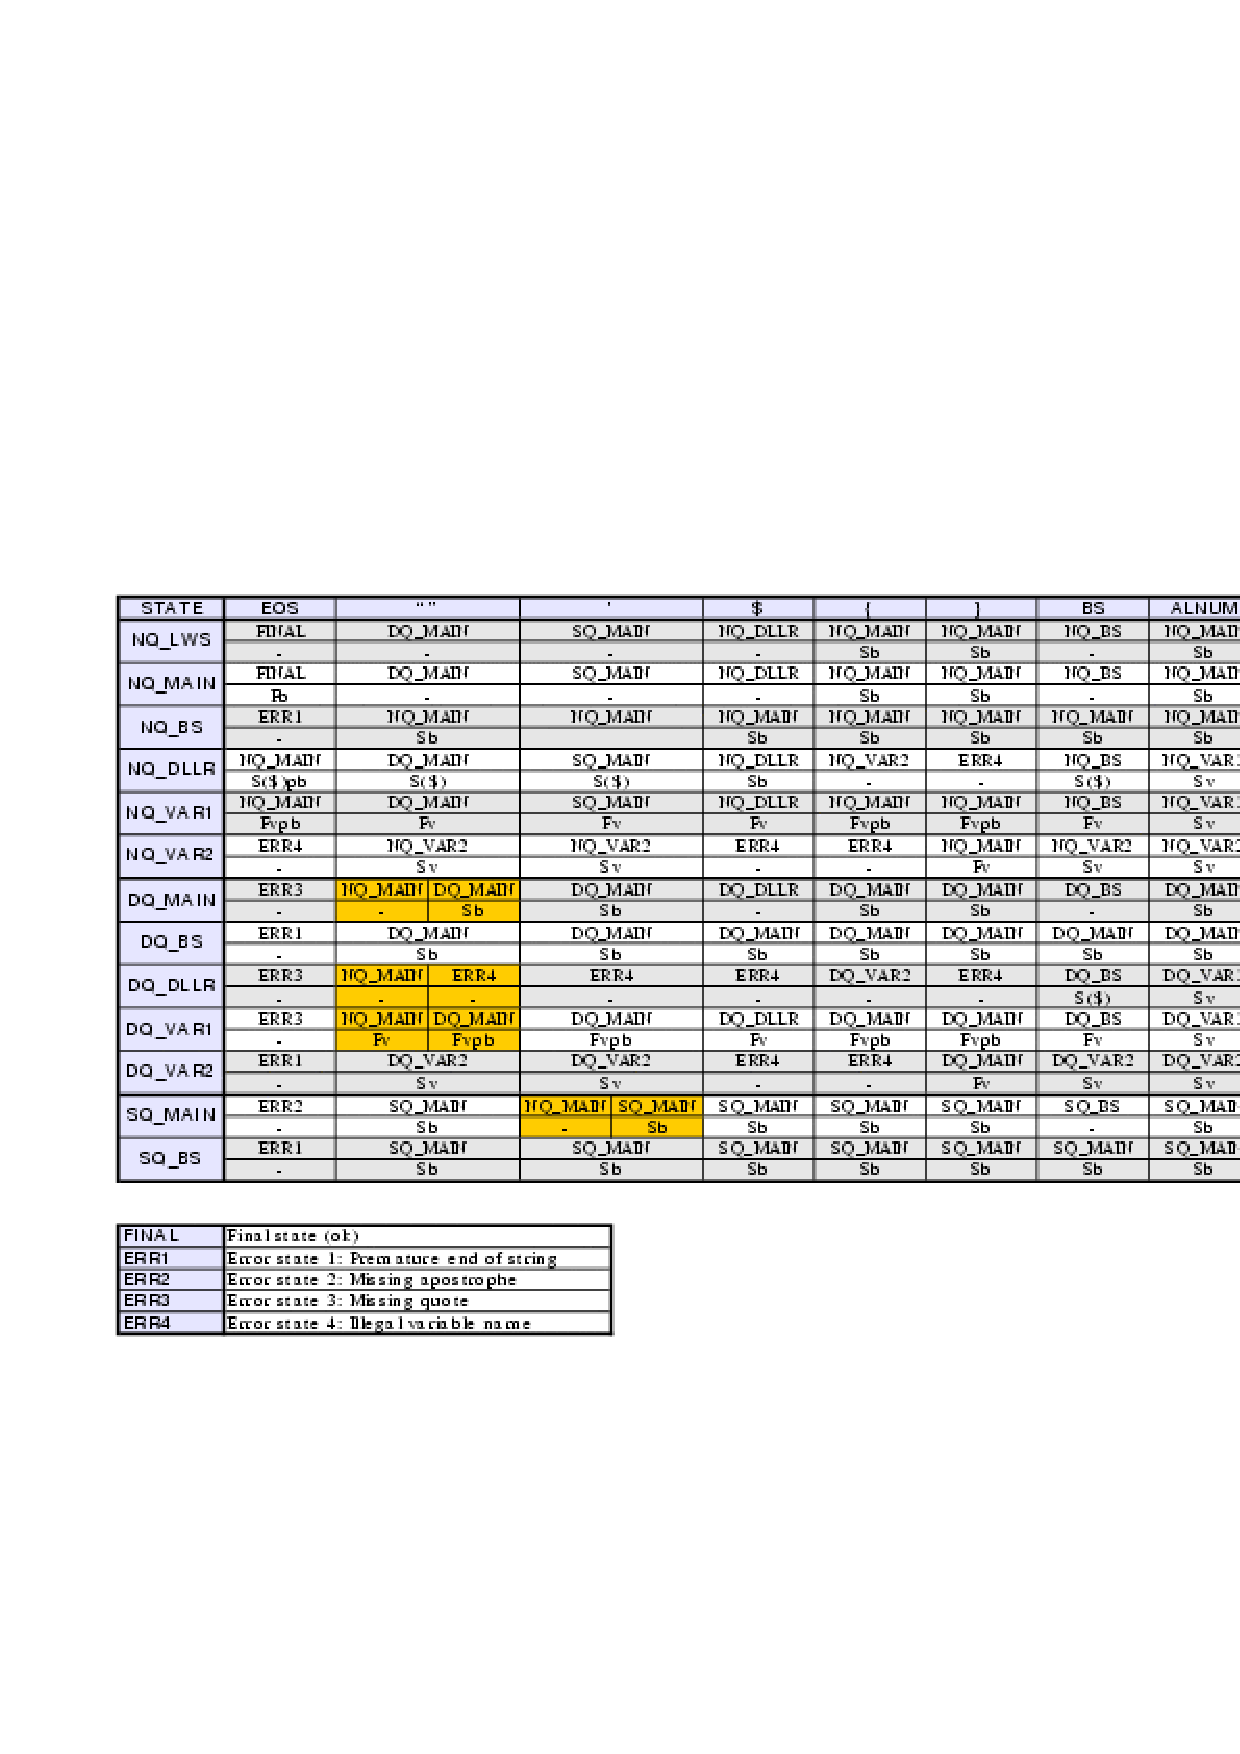
\includegraphics[scale=0.7,viewport= 0 180 792 612]{statetable}
  \caption{State transition table for the string parser.}
  \label{fig:statetable}
\end{figure}

\begin{difficult}
  Figure~\ref{fig:statetable} shows the Mealy state transitions
  automaton for parsing job strings and regular strings. The table shows
  for a given state and input character class, the resulting state and
  action.
  
  The start state for job strings is NQ\_LWS, and the left side of
  yellow states applies. The start state for regular single-quoted
  strings is SQ\_MAIN and for regular double-quoted strings DQ\_MAIN.
\end{difficult}

Multi-line strings are permitted. There are two multi-line modes. In
line-continuation mode, a backslash immediately before a linefeed
character implies that both are ignored, and the next line is viewed as
part of the current line. An unprotected newline character inside a
string will be copied into a regular string, or is a split point for job
strings. Table~\ref{tab:multiline} shows examples for the handling of
multiline strings.

\begin{table}[htbp]
  \centering
  \begin{tabular}{|p{25mm}|l|}\hline
    \textbf{Input string} & \textbf{Resulting string}\dd\hline
    1: \verb|"some \|\newline2: \verb|string"|
        & >>\verb|some string|<<\dd
    1: \verb|"some|\newline2: \verb|string"|
        & >>\verb|some\nstring|<<\dd
  \end{tabular}
  \caption{Multi-line string handling.}
  \label{tab:multiline}
\end{table}

\subsection{Format}
\label{sec:format}

The configuration file is a format free language. It does not care about
any number of (linear) whitespaces between its tokens. However, to
maintain a Unix shell like semantic, commands are auto-delimited by the
end of a line. Continuation lines are not permitted (if you don't know
what that means, you don't need it). Multiple commands in the same line
must be separated with a semicolon.

The file may contain comments in the tradition of scripting languages. A
comment starts with the hash (\#) character, and extends through the end
of the line. 

There is no filename globbing. If you need globbing (e.g. working with
wildcarded filenames as arguments), you must run your jobs through
\verb|/bin/sh -c | to let shell do the globbing for you. However, be
warned that such encapsulation will add another level of job string
de-quoting and interpretation.



\section{Commands}
\label{sec:commands}

While most commands have a rather static semantic, some permit optional
arguments. The following sections use the following generic descriptions
to denote a non-terminal token:

>>string<< is the placeholder for a string, single or double quoted.
>>id<< is the placeholder for an identifier. >>options<< is the
placeholder for a list of options. Each option is an identifier itself.
Multiple options are separated by linear whitespace. Reserved words are
not permitted as valid identifiers within an option string.



\subsection{Other commands}
\label{sec:other}

This category describes commands which deal with the configuration of
the kickstart application itself.


\subsubsection{Include}
\label{sec:include}

\begin{verbatim}
include >>string<<

include "/my/site/local.cfg"
\end{verbatim}

The configuration file permits the recursive inclusion of other
configuration files, which are specified by giving their name within the
>>string<<. Since these denote files on the remote system, this
mechanism allows for site-specific tie-ins of configuration values.
Furthermore, since a double-quoted string is subject to interpretation,
it permits for a rich flavor of dynamically determinable filesnames to
include.

If the file cannot be opened for reading by the effective user running
gridshell, its contents will be ignored. 

Included files may include other files. However, a loop-detection
mechanism is not (yet) in place, thus circular dependencies are most
likely crash gridshell with a remote resource exhaustion. 


\subsubsection{Debug}
\label{sec:debug}

Not yet implemented - debugging is currently hard-coded as seen fit. 


\subsubsection{Xmlns}
\label{sec:xmlns}

\begin{verbatim}
xmlns >>identifier<<

xmlns ptc
\end{verbatim}

The provenance tracking record (PTR) may occasionally require a
namespace identifier, if it is to be included as part of other XML
documents. Usually, you won't need to set this attribute, though. Please
note that the argument is an identifier, not a string. The rules for
valid identifiers are more restrictive, see section~\rref{sec:ident}.

Each repetition of this command will overwrite any previously configured
value.

\subsection{Descriptions}
\label{sec:descriptions}

The descriptions set up certain values to be reflected into the
provenance tracking record (PTR), the ultimate result of the gridshell.


\subsubsection{Site}
\label{sec:site}

\begin{verbatim}
site >>string<<

site 'UBuffalo'
\end{verbatim}

The string defines the name of a site. This is useful for future cases,
where a 2nd level staging mechanism accesses some form of external
replica mechanism, and needs to store a site handle. Note that the site
handle is an arbitrarily chosen name with no further meaning beyond the
GriPhyN Virtual Data System.

Each repetition of this command will overwrite the previous value. For
now, the site handle is just reflected in the PTR.



\subsubsection{Transformation}
\label{sec:tr}

\begin{verbatim}
tr >>string<< [>>string<< [..]]
transformation >>string<< [>>string<< [..]]

transformation 'voeckler::findrange:1.0'
\end{verbatim}

This command comes in two flavors, with a short and a long reserved
word. Their meaning is equivalent. The string list arguments describe a
fully-qualified VDC-definition name each. Such a name is usually
something akin to "namespace::\-name:\-version".

Each repetition of this command will append to a list of transformation
records. While there can be only one transformation that is being
called, a compound transformation may call other transformations. Thus,
the call stack is part of the record. The values are solely used to be
reflected in the PTR.

\subsubsection{Derivation}
\label{sec:dv}

\begin{verbatim}
dv >>string<<
derivation >>string<<

derivation 'voeckler::right:1.0'
\end{verbatim}

This command also comes in two reserved word flavors, which are
equivalent. The string argument describes the fully-qualified
VDC-definition name, which is usually something akin to
"namespace::name:version".

Each repetition of this command will overwrite the previous value. The
value is solely used to be reflected in the PTR. 

\subsubsection{Input}
\label{sec:input}

\begin{verbatim}
input >>lfn<< >>sfn<<
input md5 >>lfn<< >>sfn<<
input >>lfn<< >>sfn<< >>tfn<< ...
input md5 >>lfn<< >>sfn<< >>tfn<< ...

input 'voeckler.f.a' '/home/voeckler/vdldemo/voeckler.f.a'
\end{verbatim}

Each repetition of this command will register a logical filename (LFN)
with a storage filename (SFN). Additionally, if 2nd level staging is
required, any number of input transfer filenames (iTFN) may be
associated. For each LFN, only one SFN can be associated. For each SFN,
multiple iTFNs may be associated. All of LFN, SFN and TFN are strings,
and thus must be enclosed in quotes.

Effectively, for each registered input filename, a stat record will be
obtained from the SFN after gridshell parsed all its arguments and ran
an optional 2nd level stage-in job (see~\rref{sec:stagein}). The stat
record is obtained \emph{before} any of the regular subjobs pre through
cleanup are being run.

The information from the stat call is being reflected into the PTR, one
record for each file, featuring the LFN as distinction. Files may appear
in both, the input and the output list.

The optional argument \verb|md5| specifies that an MD5 sum should be
obtained of the file, and become part of the resulting stat info record.
Note that \verb|md5| is an option, and thus not quoted.

\subsubsection{Output}
\label{sec:output}

\begin{verbatim}
output >>LFN<< >>SFN<<
output md5 >>LFN<< >>SFN<<
output >>LFN<< >>SFN<< >>TFN<< ...
output md5 >>LFN<< >>SFN<< >>TFN<< ...

output md5 'voeckler.f.d' '/home/voeckler/vdldemo/voeckler.f.d'
\end{verbatim}

Each repetition of this command will register a logical filename LFN
with a storage filename SFN. Additionally, if 2nd level staging is
required, any number of output transfer filenames oTFN may be
associated. For each LFN, only one SFN can be associated. For each SFN,
multiple oTFNs may be associated. All of LFN, SFN and TFN are strings,
and thus must be enclosed in quotes.

Effectively, for each registered output filename, a stat record will be
obtained from the SFN after gridshell ran all jobs, but before the
optional 2nd level stage-out job is run (see section 2.4.y).

The information from the stat call is being reflected into the PTR, one
record for each file, featuring the LFN as distinction. Files may appear
in both, the input and the output list.

The optional argument \verb|md5| specifies that an MD5 sum should be
obtained of the file, and become part of the resulting stat info record.
Note that \verb|md5| is an option, and thus not quoted.


\subsection{Processing Environment}
\label{sec:processing}

The processing environment deals with setting up the environment in
which jobs (see~\rref{sec:jobs}) are being run. The changes pertain only
to gridshell, and stay within gridshell.


\subsubsection{Set}
\label{sec:set}

\begin{verbatim}
set >>id<< >>string<<

set PATH "$PATH:$HOME/bin"
\end{verbatim}

The set command is similar to the C-shell \texttt{setenv} command. The
identifier >>id<< denotes a key in the Unix environment, which is to be
set to the specified value of >>string<<. Please note that the string,
if double-quoted, may be subject to variable interpolation.

Enviroment setting are \emph{not} reflected in the PTR. The environment
variables are changed during compile-time. Environment values are
overwritten, if they already exist.


\subsubsection{Chdir}
\label{sec:chdir}

\begin{verbatim}
chdir >>string<<
chdir create >>string<<

chdir create "/home/$LOGNAME/vdldemo/tmp"
\end{verbatim} 
%$
The chdir command determines the current working directory. The command
comes in two flavors, with and without the \emph{create} option.

Without the \emph{create} option, the specified working directory is
attempted to be created before changing into it. Failure to create the
directory through reason of existence will be ignored. Other failures on
the mkdir command will cause a semantic error during compile-time.

Regardless of options, in the next step, gridshell will attempt to
change into the specified working directory. If the change fails, the
previous current workding directory remains current. The working
directory is changed during compile-time. Effects are immediate on
relative filenames.

If no chdir command is specified whatsoever, the gridshell uses the
working directory assigned by the scheduling system, i.e. where it was
started in. The current working directory will be reflected in the PTR. 

Multiple specificiations will change the directory again and again. The
finally chosen working directory is recorded in the PTR. 

\subsubsection{Feedback}
\label{sec:feedback}
\begin{verbatim}
feedback >>string<<
feedback >>id<< >>string<<

feedback ATLAS_FEEDBACK "/dev/shm/atlas-XXXXXX"
feedback 'gs-fb-XXXXXX'
\end{verbatim}

The feedback is currently a simple mechanism to allow gridshell-aware
applications to send appli\-ca\-tion-specific data back to the submit host.
Any processing, collection or visualization of this data is up to the
user application framework.

The >>id<< specifies the name of an environment variable which is to be
set to the filename of the named pipe (FIFO). If no identifier is
specified, the default of \texttt{GRIDSTART\_CHANNEL} is used.

The filename is created using the mkstemp(2) system call from the
pattern provided by the string. The filename string \emph{must} have a
suffix of six capitol \texttt{X} letters, or these letters will be
mandatorily appended, including a separating hyphen.

If the filename is absolute, starting is a slash, the specified path
will be used. If the filename is relative, not starting with a slash, an
appropriate temporary directory will be determined and prefixed.

The gridshell attempts to create a FIFO (Unix named pipe) from the
pattern with the temporary filename. It changes the environment to
record the filename, so that subjobs (see~\rref{sec:jobs}) may write to
this channel.

[future lab: Permit any number of such channels, and multiplex them]

If feedback is specified multiple times, only the last specification
will persist. Previous channels will be closed and removed. The feedback
mechanism is only activated, if the feedback was specified at least
once. The chosen FIFO and its stat information is part of the standard
statinfo PTR record.


\subsubsection{Stdin}
\label{sec:stdin}

\begin{verbatim}
stdin >>string<<
stdin here >>string<<

stdin 'my/file'
stdin here 'copy to stdin'
\end{verbatim}

These directives permit the connection of the stdin filehandle of
subjobs with an existing file. The primary use of this option is to
peruse input, if any stdin pertains to a GVDS-tracked file during a
computation. Ideally, only the main computational jobs should access
these files.

You can (currently) only use one redirected stdio for all subjobs. Thus,
if you redirect stdin to a file, this file will be used for all subjobs.

Will the file be reopened for each job? Depending on what you connect
your stdin to, the answer is yes and no. Please refer to
table~\ref{tab:stdin} for the different open modes. The reason a regular
file is being reopened lies in the fact that an open filedescriptor is
not maintained between jobs. Furthermore, the last position of the file
cannot be remembered, because it cannot be obtained: The file handle of
a regular file, once opened, will be passed completely into the job's
application space.

\begin{table}[htb]
  \centering
  \begin{tabular}{|r|p{80mm}|}\hline
    \textbf{file type} & \textbf{reuse or reopen mode}\dd\hline
    regular file & file will be reopened for each job.\dd
    file descriptor & file descriptor will be dupped.\dd
    temporary file & same as file descriptor.\dd
    here document & same as file descriptor.\dd
    user FIFO & not applicable, but same as descriptor.\dd
  \end{tabular}
  \caption{Open modes for \emph{stdin}.}
  \label{tab:stdin}
\end{table}

The special filename of just a hyphen means to connect the filehandle
with the one passed to the gridshell. However, in order to use a
\emph{here document}, which copies content from the configuration onto
the stdin of the application, you must use the \texttt{here} option.

When using the \texttt{here} option, the string is not a filename, but
the content to be put into a temporary file, which is subsequently
connected with the stdin of the jobs. Multi-line strings are valid, and
regular string interpolation applies, see section~\rref{sec:strings}.

[future lab: Add options to allow disassociation of stdio handles during
stage jobs. Add options to permit disassocation during non-main job.]
 
A stdin redirection should only be specified once. A re-configuration
will close a previous configuration.

Default for stdin is to connect to \verb|/dev/null| in the absence of
any specification.


\subsubsection{Stdout and Stderr}
\label{sec:stdout}\label{sec:stderr}

\begin{verbatim}
stdout >>string<<
stdout append >>string<<
stdout truncate >>string<<

stderr >>string<<
stderr append >>string<<
stderr truncate >>string<<

stdout '-'
stderr append 'local.err'
\end{verbatim}

These directives permit the connection of stdio filehandles of subjobs
with existing files. The primary use for these options is to capture
output, if any stdout or stderr pertains to a GVDS-tracked file during a
computation. Ideally, only the main computational jobs should access
these files. However, you should keep in mind that various error
conditions may result in output to stderr for failures of other subjobs.

You can (currently) only use one redirected stdio for all subjobs. Thus,
if you redirect stdout into a file, this file will be used for all
subjobs.

Default mode for these directives is the truncated mode. In truncate
mode, a previously (before the start of the gridshell) existing file is
truncated at compile-time. In append mode, a previously existing file is
opened for appending.

The special filename of just a hyphen means to connect the filehandle
with the one passed to the gridshell. 

[future lab: Add options to allow disassociation of stdio handles during
 stage jobs. Add options to permit disassocation during non-main job.]

Each stdio redirection should only be specified once. A re-configuration
will close and overwrite a previous setup. 

Default for stdout and stderr is to connect to separate temporary files
in the absence of any specification. The first page of data from the
temporary files are reflected in the stat info records of the PTR for
stdout and stderr.


\subsection{Job commands}
\label{sec:jobs}

The job configurations describe the command and command line to be used
for subjobs. All specifications are optional except for the main job,
which must be specified.

The chaining of job results is loosely as follows: 

\begin{enumerate}
\item run stage-in job, if applicable
\item obtain stat records on files declared input
\item run setup job chain
\item run pre job chain \texttt{\&\&} run main job \texttt{\&\&} run
  post job chain
\item run cleanup job chain
\item obtain stat records on files declared output
\item run stage-out job, if applicable
\end{enumerate}

If any prejob exists and fails, no further jobs in the pre, main, post
chain will be run. If the main job fails, no further jobs in the post
chain will be run. If any of the postjobs fails, the chain will not be
continued. The stagein, stageout, setup and cleanup jobs are independent
of any failures in the pre chain, main job, and post chain.

Any number of setup, pre, post and cleanup jobs may be specfied. They
are queued into separate chains, and each chain executes its jobs in the
order of their specification.

The main job is mandatory. It must be specified once, and should be
specified once only. Multiple specifications will overwrite previous
ones. 

Please note the commandline specification string for jobs is subject to
double interpretation, once during compile-time, and once during
run-time, see~\rref{sec:strings} for details.

[future lab: Drop the double interpolation -- too confusing. It is an
artefact of code recycling]\newline{}[Is it already dropped?]
 
The stdio of any job will be connected according to the specification of
stdin, stdout and stderr, see~\rref{sec:processing}. Stdin defaults to
\verb|/dev/null|, stdout to a temporary file, and stderr to a different
temporary file.

Absolute application names are taken at face value, and may fail in
their non-existence. Relative names are canonified with the help of the
current working directory. [fixme: are they?]

\subsubsection{Setup Jobs}
\label{sec:setup}

\begin{verbatim}
setup >>string<<

setup "/bin/mkdir -p $HOME/tmp"
\end{verbatim}

The setup job configuration may be specified multiple times. Each job
will be queued into a chain \emph{setup}, and at run-time, these will be
executed in the order of their chaining. Any setup job may fail without
affecting any other jobs.

Note: Usually you are better of wrapping even simple commands into a
real shell script, set the execute bit on it, and run just that
particular shell script.


\subsubsection{Pre Jobs}
\label{sec:pre}

\begin{verbatim}
pre >>string<<

pre '/bin/date'
pre '/usr/bin/env perl -i.bak -pe \\"s{a}{b}g\\" *.jof'
\end{verbatim}

The pre job configuration may be specified multiple times. Each job will
be queued into a chain \emph{prejobs}, and at run-time, these will be
executed in the order of their chaining. The first failed prejob will
result in a failed execution of the computation. No further prejobs, no
main jobs, and no postjobs will be run in case of failure.

\subsubsection{Main Job}
\label{sec:main}

\begin{verbatim}
main >>string<<

main 'computation.sh'
\end{verbatim}

The main job must be specified, and should only be specified once. A
minimum configuration file contains at least a configuration for the
main job. If the main job fails, all will be assessed as failure. No
post jobs will be run in case of failure.

\subsubsection{Post Jobs}
\label{sec:post}

\begin{verbatim}
post >>string<<

post '/bin/date'
\end{verbatim}

The post job configuration may be specified multiple times. Each job
will be queued into a chain \emph{postjobs}, and at run-time, these will
be executed in the order of their chaining. The first failed postjob
will result in a failed execution of the computation. No further
postjobs will be run in case of failure.


\subsubsection{Cleanup Jobs}
\label{sec:cleanup}

\begin{verbatim}
cleanup >>string<<

cleanup 'rm *.log'      # this will NOT work: ENOENT
cleanup '/bin/sh -c \'rm *.log\''       # this might work
\end{verbatim}

The cleanup job configuration may be specified multiple times. Each job
will be queued into a chain \emph{cleanup}, and at run-time, these will
be executed in the order of their chaining. Any cleanup job may fail
without affecting any other jobs.

Note: Usually you are better of wrapping even simple commands into a
real shell script, set the execute bit on it, and run just that
particular shell script.


\subsection{Optional 2nd-level Staging}
\label{sec:staging}

The stageout and stagein jobs are optional, should only be specified
once. The job restriction and feature, as shown in section 2.4, apply
also to stage jobs. Multiple specifications of stage jobs will overwrite
previous specifications.

[future lab: Do we need multiple stage call-outs?]

The stage jobs deal with the 2nd level staging of files. The 2nd level
staging comes into effect, if a compute cluster does not share a
filesystem between the externally visible storage element, and the
internal worker node. The 2nd level staging may be employed in this case
to transfer input files to the worker node before any computation takes
place, and to store output files to the storage element after any
computation took place.

Stage jobs have an invisible final argument. The final argument is
dynamically affixed. It is the name of a temporary file which contains a
list of file mapping from SFN to TFN. The format is determined by the
format string, which is the first argument string to the stage commands.

The format string may contain three kinds of placeholders, each of which
may occur multiple times:

\begin{center}
  \begin{tabular}{|l|p{100mm}|}\hline
    \textbf{fmt} & \textbf{meaning}\dd\hline
    \texttt{\%l} & replaced with the LFN\dd
    \texttt{\%s} & replaced with the SFN\dd
    \texttt{\%t} & shortcut for \texttt{\%t\{ \}}\dd
    \texttt{\%t\{x\}} & replaced with the TFN list. The string x is the
    separator, if more than one TFN is available\dd
  \end{tabular}
\end{center}

The concrete interface is up to the user, and the interface with
external application called out to. Note that curly braces may not be
part within the separator string x. Also, leaving the separator string
away defaults to a single space separator. Use double-quoted strings, if
you intend to use $\backslash{}r\backslash{}n$. Some popular examples
include:

\begin{verbatim}
'%s %t'               single-line: SFN -> TFN1 TFN2 ..
"%l %s %t{\r\n+ }"    multi-line: use continuation symbol
"%s %t{\r\n%s }"      multi-line: repeat SFN for each TFN
\end{verbatim}

A CRLF will be implicitely appended to the end of the format string. The
author of gridshell is aware that filenames with spaces inside them, as
frequently seen on MACs and now on Windows, will break the interface.
[fixme: we may/will need quoting].

In order to create the list of files, the input and output configuration
commands must use the three argument version, which associates a TFN
with an LFN. 


\subsubsection{Stagein}
\label{sec:stagein}

\begin{verbatim}
stagein >>string<< >>string<<

stagein "%s %t" 'transfer.sh -I'        # make sure to have x bit set
\end{verbatim}

The stagein job specification, if present, specifies a script or callout
to run for the 2nd level stage-in of files. The final argument will be
dynamically attached, and is the name of a file containing a list of
files mappings.

No stagein job will be run, if the list of stagable input files is
empty. If two argument input configuration was used, i.e. the TFN is
missing for an SFN, this file will not become part of the list.


\subsubsection{Stageout}
\label{sec:stageout}

\begin{verbatim}
stageout >>string<< >>string<<

stageout "%s %t" 'transfer.sh -O'        # ensure x bit
\end{verbatim}

The stageout job specification, if present, specifies a script or
callout to run for the 2nd level stage-out of files. The final argument
will be dynamically attached, and is the name of a file containing a
list of files mappings.

No stage-out job will be run, if the list of stagable output files is
empty. If two argument output configuration was used, i.e. the TFN is
missing for an SFN, this file will not become part of the list.




\section{Results}
\label{sec:results}

The gridshell [...]


\subsection{The Provenance Tracking Record}
\label{sec:ptr}

The provenance tracking record written by the gridshell is transported
on \emph{stdout} made available by the remote scheduler. Since the
provenance tracking record will be compiled and written after all jobs
were run, it is usually a good idea, when using Globus, to disconnect
the stdout, and transfer results at the end-of-(Globus-)job. This will
save filehandle resources and other kernel resources on the gatekeeper
host.

The provenance tracking record contains a variety of information,
usually more than will be stored in the provenance tracking catalog
(PTC). Much of the information is useful for debugging, too. 

Some remote scheduling systems protocol their own information on the
stdout. Furthermore, if subjobs are configured to use gridshell's stdout
handle, their output may also appear on this handle. While the PTR is
distinct in this mix of data, dissemination and multiplexing of stdout
is not a task that can be solved by a gridshell. 

The provenance tracking record (also known as invocation records), can
be found online. Please refer to \verb| http://www.griphyn.org/workspace/VDS/|.

\subsection{The Feedback Channel}
\label{sec:channel}

The feedback channel is transported via stderr filehandle to the submit
host. Since feedback information is immediate, Globus-IO streaming mode
is applicable for this channel. However, Globus streaming is a best
effort operation: Remote scheduling systems may decide to \emph{not}
make the stderr available until after the job is done. There is no
guarantee that stderr will actually be streamed, or stream continually.

The gridshell tries to use the stderr for application feedback. The
gridshell feedback records are XML encapsulated chunks to distinguish
them from other noise on the stderr channel.


\subsubsection{Exponentially Backed-off Heartbeat}

The gridshell wakes up at regular intervals to check on various
filehandles and the system state. At exponentially growing intervals,
gridshell will check that it could actually kill its child. The result
will be send as feedback chunk with a channel number of zero:

\begin{verbatim}
<chunk channel="0" size="23" when="2004-02-03T16:38:18.806-06:00">
<![CDATA[heartbeat 1: 30.005 0/0]]></chunk>
\end{verbatim}

The first heartbeat is registered after 30 seconds, with the interval
doubling each time.

[fixme: grow not quite so fast, but faster than linear]


\subsubsection{Gridshell-aware Applications}

If an application is gridshell-aware, it can use the FIFO created by the
feedback configuration to send back application data. The data will be
collected in the submit host's stderr file for the job. The name of the
FIFO is determined by the identifier of the environment variable. Thus,
this mechanism can even be used in shell scripts, e.g. contain a line
like: 

\begin{verbatim}
echo "some comment" >> $GRIDSHELL_CHANNEL
\end{verbatim}

The application data will be chunked into XML, e.g:

\begin{verbatim}
<chunk channel="1" size="12" when="2004-02-03T16:48:28.068-06:00">
<![CDATA[some comment]]></chunk>
\end{verbatim}

The chunking borders are arbitrary, and outside the sphere of influence
of the gridshell. Never assume that data written in one write will
result in one chunk, nor assume that data separately written data will
result in multiple chunks.

Worse, there is currently the limitation that only one writer at each
time should write to the feedback channel. Since it is a mostly untested
feature, there may still be bugs involved, which may lead to the
premature cancellation of a compute jobs. Thus, please test before
relying on production.



\end{document}
%%% Local Variables: 
%%% mode: latex
%%% TeX-master: t
%%% End: 
